\documentclass[12pt,letterpaper]{article}

\usepackage{amsfonts}
\usepackage{graphics}
\usepackage{graphicx}
\usepackage{colortbl}
\usepackage{amsmath}

\usepackage{algorithm}
\usepackage[noend]{algpseudocode}
\usepackage{array}

\usepackage{epstopdf}

\setlength\intextsep{10pt}
\setlength\textfloatsep{10pt}

\newenvironment{proof}{\noindent{\bf Proof:}}{\qed\bigskip}

\newtheorem{theorem}{Theorem}
\newtheorem{corollary}{Corollary}
\newtheorem{lemma}{Lemma} 
\newtheorem{claim}{Claim}
\newtheorem{fact}{Fact}
\newtheorem{definition}{Definition}
\newtheorem{assumption}{Assumption}
\newtheorem{observation}{Observation}
\newtheorem{example}{Example}
\newcommand{\qed}{\rule{7pt}{7pt}}

\newcommand{\assignment}[4]{
\thispagestyle{plain} 
\newpage
\setcounter{page}{1}
\noindent
\begin{center}
\framebox{ \vbox{ \hbox to 6.28in
{\bf CS578/STAT590: Introduction Machine Learning \hfill #1}
\vspace{4mm}
\hbox to 6.28in
{\hspace{2.5in}\large\mbox{Problem Set #2}}
\vspace{4mm}
\hbox to 6.28in
{{\it Handed Out: #3 \hfill Due: #4}}
}}
\end{center}
}

\newcommand{\solution}[4]{
\thispagestyle{plain} 
\newpage
\setcounter{page}{1}
\noindent
\begin{center}
\framebox{ \vbox{ \hbox to 6.28in
{\bf CS578/STAT590: Introduction to Machine Learning \hfill #4}
\vspace{4mm}
\hbox to 6.28in
{\hspace{2.5in}\large\mbox{Problem Set #3}}
\vspace{4mm}
\hbox to 6.28in
{#1 \hfill {\it Handed In: #2}}
}}
\end{center}
\markright{#1}
}



\def\Comment#1{\textsf{\textsl{$\langle\!\langle$#1\/$\rangle\!\rangle$}}}



\oddsidemargin 0in
\evensidemargin 0in
\textwidth 6.5in
\topmargin -0.5in
\textheight 9.0in

\begin{document}

\solution{Gen Nishida}{\today}{3}{Fall 2014}
% Fill in the above, for example, as follows:
% \solution{John Smith}{\today}{1}{Fall 2014}

\pagestyle{myheadings}  % Leave this command alone

\section{Questions}

\begin{enumerate}
\item Fitting an SVM classifier by hand (source: Machine Learning, a probabilistic perspective. K Murphy)

\begin{enumerate}
\item Write down a vector that is parallel to the optimal vector w.

The decision boundary is perpendicular to the vector $\phi(x_2)-\phi(x_1)$.
\[
\phi(x_2)-\phi(x_1)=[1, 2, 2]^T-[1, 0, 0]^T=[0, 2, 2]^T
\]
Thus, the vector that is parallel to the optimal vector $w$ is $[0, 1, 1]^T$.

\item What is the value of the margin that is achieved by this $w$?

The maximum margin is the half of the distance between two points in the 3d feature space. Thus,
\[
\frac{\|\phi(x_2)-\phi(x_1)\|}{2}=\frac{\|[0, 2, 2]^T\|}{2}=\sqrt{2}
\]

\item Solve for $w$, using the fact the margin is equal to $1/\|w\|$.

Let $w=k [0, 1, 1]^T$. Then,
\[
\|w\|=k\|[0, 1, 1]^T\|=\sqrt{2}k
\]
Since the margin is $\sqrt{2}$,
\[
\sqrt{2}=\frac{1}{\|w\|}=\frac{1}{\sqrt{2}k}
\]
By solving this, we obtain $k=1/2$. Thus, $w=[0, 1/2, 1/2]^T$.

\item Solve for $w_0$ using your value for $w$ and Equations 1 to 3.

By substituting $w$ of Equations 2 and 3, we get
\[
\begin{cases}
y_1(w^T\phi(x_1)+w_0)=-([0, 1/2, 1/2]^T \cdot [1, 0, 0]^T+w_0)=-w_0\ge 1 \\
y_2(w^T\phi(x_2)+w_0)=([0,1/2,1/2]^T \cdot [1, 2, 2]^T+w_0)=2+w_0\ge 1
\end{cases}
\]
By solving this, we obtain
\[
-1\le w_0 \le -1
\]
Thus, $w_0=-1$.

\item Write down the form of the discriminant function $f(x)=w_0+w^T\phi(x)$ as an explicit function of $x$.

\[
f(x)=w_0 + w^T \phi(x)=-1 + [0, 1/2, 1/2]^T \cdot [1, \sqrt{2}x, x^2]^T=\frac{1}{2}x^2+\frac{1}{\sqrt{2}}x-1
\]

\end{enumerate}

\item We define a concept space C that consists of the union of $k$ disjoint intervals in a real line. A concept in C is represented therefore using $2k$ parameters: $a_1 \le b_1 \le a_2 \le b_2 \le \cdots \le a_k \le b_k$. An example (a real number) is classified as positive by such concept iff it lies in one of the intervals. Give the VC dimension of H (and prove its correctness).

The answer is $2k$.

{\bf Proof:}

Let $VC(k)$ be the VC dimension for $k$ disjoint intervals in a real line. I prove by indiction that $VC(k)=2k$ in the following. When $k=1$, two examples have four patterns in total, and all the cases can be correctly classified (Figure \ref{fig:vc_dimension1}). Thus, $VC(1)=2$, which satisifies the above hypothesis. 

\begin{figure}[hbtp]
\centering
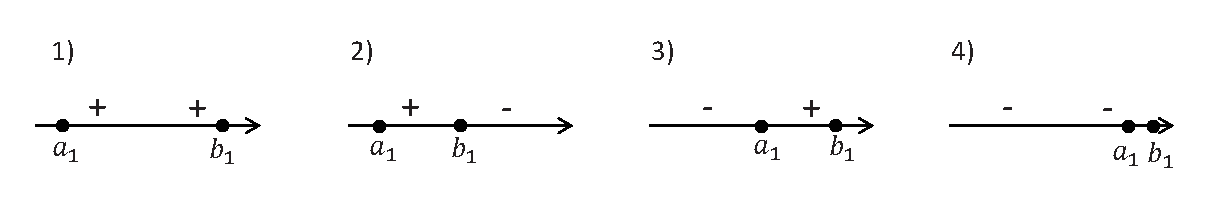
\includegraphics[width=150mm]{vc_dimension1}
\caption{For the case of $k=1$, two examples are correctly classified in all the four cases. Thus, $VC(1)=2$.}
\label{fig:vc_dimension1}
\end{figure}

Now, given that $VC(k-1)=2(k-1)$, we want to show that two additional examples can be correctly classified by an additional interval. Assume without loss of generality that two additional numbers are greater than the existing $2(k-1)$ ones that are already classified. Then, there are only four cases in terms of the labels of two additional examples, and they are correctly classified by $k$-th interval in all cases (Figure \ref{fig:vc_dimension2}). 
\begin{figure}[hbtp]
\centering
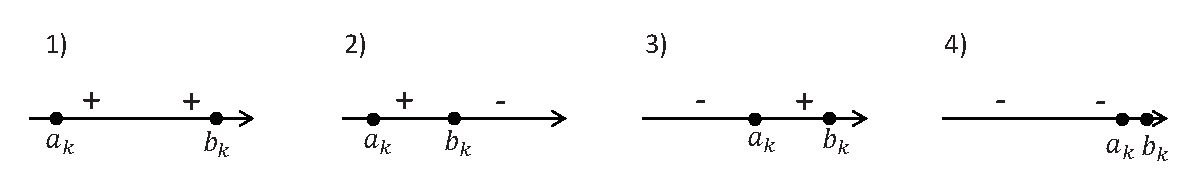
\includegraphics[width=150mm]{vc_dimension2}
\caption{When adding $k$-th interval, two additional examples are correctly classified in all the four cases.}
\label{fig:vc_dimension2}
\end{figure}

Thus, 
\[
VC(k) \ge VC(k-1)+2=2(k-1)+2=2k
\]
Therefore, $VC(k)$ is at least $2k$ by induction. Also, Figure \ref{fig:vc_dimension3} shows a case in which $k+1$ positive examples and $k$ negative examples cannot be correctly classified. Thus, $VC(k) < 2k+1$. This concludes $VC(k) = 2k$.
\begin{figure}[hbtp]
\centering
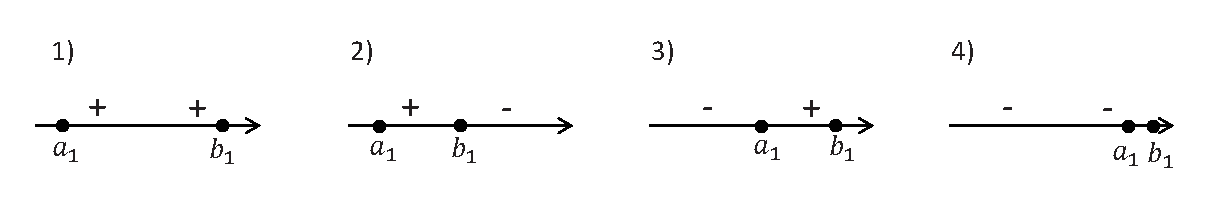
\includegraphics[width=140mm]{vc_dimension3}
\caption{This figure shows a case in which $k+1$ positive examples and $k$ negative examples cannot be correctly classified by $k$ disjoint intervals. The right most positive example (red color) is classified incorrectly. Thus, $VC(k) < 2k+1$.}
\label{fig:vc_dimension3}
\end{figure}


\item The Gradient Descent (GD) algorithm

\begin{enumerate}
\item Write in one sentence: what are the hyper parameters of the GD algorithm.

The hyper parameters are 1) how to define the initial parameters: initializing 0 or randomly, 2) the learning rate that is the step size of updating the parameters, and 3) the convergence criteria when to stop the iteration such as the maximum number of iterations and a threshold to judge whether it is coverged.

\item Write in one sentence: What is the difference between $l1$ and $l2$ regularization.

$l1$ regularization uses $l1$ norm of $w$ as the regularization term, which encourages the sparsity and leads to a simpler model, while $l2$ regularization uses $l2$ norm of $w$.

\item Write down the gradient descent algorithm applied to hinge loss with $l2$ regularization.

\begin{algorithm}
\caption{Gradient descent algorithm applied to hige loss with l2 regularization}\label{euclid}
\begin{algorithmic}[1]
\Procedure{HingeRegularizedGD()}{}
\State $w=(0, \cdots, 0)$
\State $b=0$
\For{$i=0$ to $maxIterations$}
\State $\Delta w=(0, \cdots, 0)$
\State $\Delta b=0$
\ForAll{training data $(x_d, y_d)$ for $d = 1,\cdots,D$}
\If{$y_d (w \cdot x_d + b) \le 1$}
\State $\Delta w= \Delta w+y_d x_d$
\State $\Delta b=\Delta b+y_d$
\EndIf
\EndFor
\State $\Delta w=\Delta w - \lambda w$
\State $w=w+\eta \Delta w$
\State $b=b+\eta \Delta b$
\EndFor
\State \Return $w$ and $b$
\EndProcedure
\end{algorithmic}
\end{algorithm}

The objective function is
\[
F(w)=\frac{\lambda}{2}\|w\|^2+\sum_i \max{(0, 1-y_i (w^Tx_i+b))}
\]
Then, its partial derivative with regard to $w$ and $b$ are
\[
\frac{\partial F(w)}{w}=\lambda w+ \sum_i
\begin{cases}
-y_i x_i & ({\rm if} \; y_i(w^Tx_i+b) \le 1) \\
0 & {\rm Otherwise}
\end{cases}
\]
and
\[
\frac{\partial F(w)}{b}=\sum_i
\begin{cases}
-y_i & ({\rm if} \; y_i(w^Tx_i+b) \le 1) \\
0 & {\rm Otherwise}
\end{cases}
\]

The algorithm is shown in Algorithm 1.

\end{enumerate}

\end{enumerate}

\section{Programming Assignment}

For the programming assignment, I used SVM with the hinge loss function and $l1$ or $l2$ regularization as required. The pseudo code of gradient descent algorithm to solve this is shown in Algorithm 2, which is basically similar to Algorithm 1 except that both $l1$ and $l2$ are supported.

\begin{algorithm}
\caption{Gradient descent algorithm applied to hige loss with l1 and l2 regularization}\label{euclid}
\begin{algorithmic}[1]
\Procedure{GD(maxIterations, regularization, $\eta$, $\lambda$)}{}
\State $w=(0, \cdots, 0)$
\State $b=0$
\For{$iter=0$ to $maxIterations$}
\State $\Delta w=(0, \cdots, 0)$
\State $\Delta b=0$
\ForAll{training data $(x_d, y_d)$ for $d = 1,\cdots,D$}
\If{$y_d (w \cdot x_d + b) \le 1$}
\State $\Delta w= \Delta w+y_d x_d$
\State $\Delta b=\Delta b+y_d$
\EndIf
\EndFor
\If{regularization == $l1$}
\For{$i=0$ to $N$}
\If{$w_i \ge 0$}
\State $\Delta w_i=\Delta w_i-\lambda$
\Else
\State $\Delta w_i=\Delta w_i+\lambda$
\EndIf
\EndFor
\ElsIf{regularization == $l2$}
\State $\Delta w=\Delta w - \lambda w$
\EndIf
\State $w=w+\eta \Delta w$
\State $b=b+\eta \Delta b$
\State \Return $w$ and $b$ if they are converged
\EndFor
\State \Return $w$ and $b$
\EndProcedure
\end{algorithmic}
\end{algorithm}

\subsection*{Feature Set}
For the continuous values, I used all the intervals between two consequtive thresholds as attributes. For instance, if an original attribute $a$ has three thresholds ${1, 2, 3}$, then the corresponding attributes will be $\{(a<1),(a\ge 1; a<2),(a\ge 2; a<3),(a\ge 3)\}$. Also, I ignored the examples that contain missing values.

\subsection*{Hyper Parameters}
There are five hyper parameters, $maxIterations$, $l1$ or $l2$, $stepSize$, $lambda$, and feature set. Unlike Perceptron algorithm, we want to minimize the objective function without worrying about overfitting because the regularization term takes care of it. Thus, I used a very large number for maxIterations, say 20000, to get the gradient descent converged. Also, as it is shown in Algorithm 2, I checked the decrease in the objective function during the gradient descent and if it is within the threshold, the gradient descent stops. I used 0.0001 as threshold. Figure \ref{fig:gradient_descent} ($featureSet=1$, $stepSize=0.001$, and $labmda=0.4$) and \ref{fig:gradient_descent_large_lambda_1} ($featureSet=2$, $stepSize=0.001$, and $labmda=1.0$) show the decrease of the objective function over the iterations. A large $stepSize$ leads to more oscillation while a small $stepSize$ requires a large number of iterations to converge. The result of Figure \ref{fig:gradient_descent} indicates that $maxIterations=20000$ is enough to converge even for a very small $stepSize$ for this problem.

\begin{figure}[hbtp]
\centering
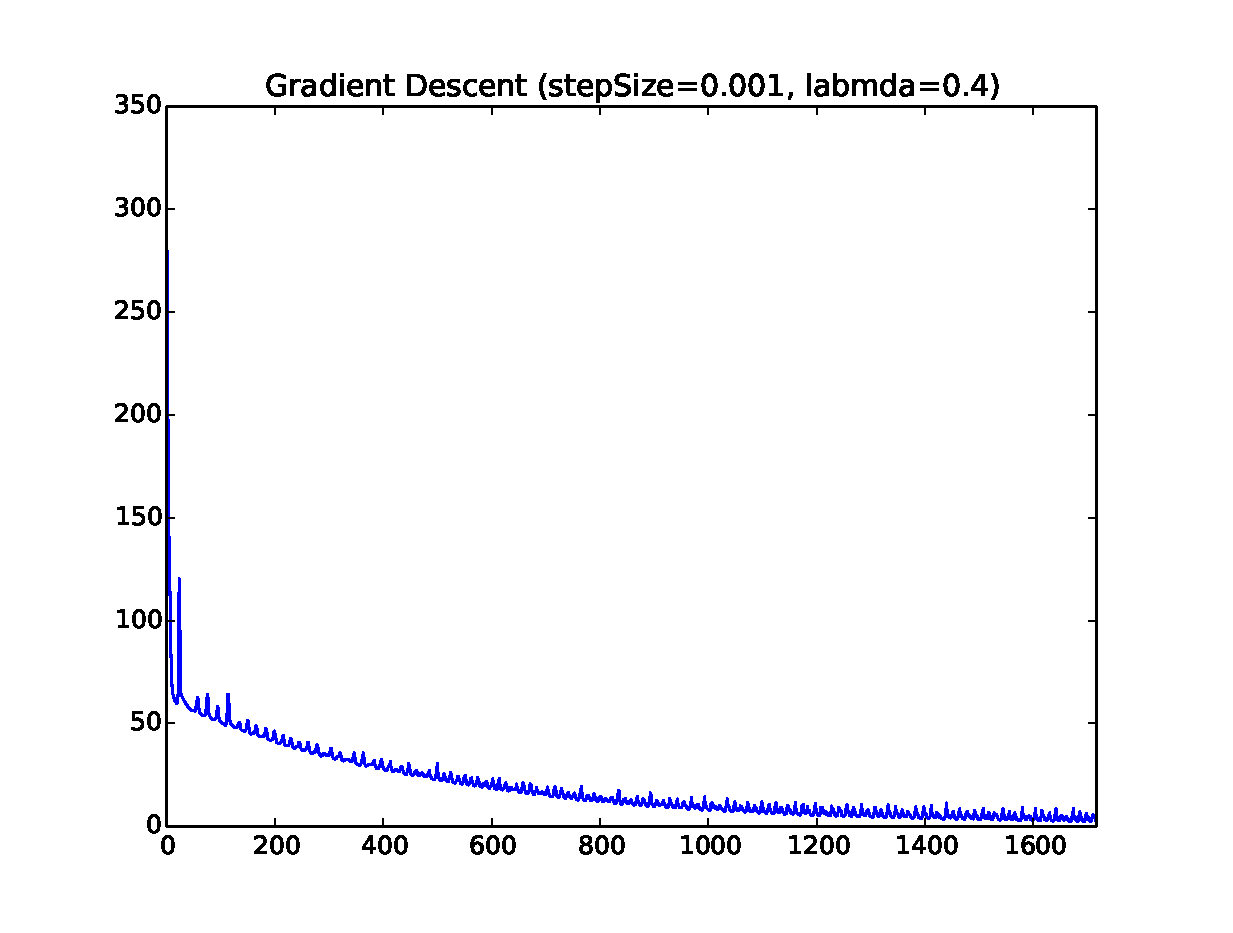
\includegraphics[width=120mm]{gradient_descent}
\caption{This figure shows the descrese of the objective over the iterations when $featureSet=1$, $stepSize=0.001$, and $labmda=0.4$.}
\label{fig:gradient_descent}
\end{figure}

\begin{figure}[hbtp]
\centering
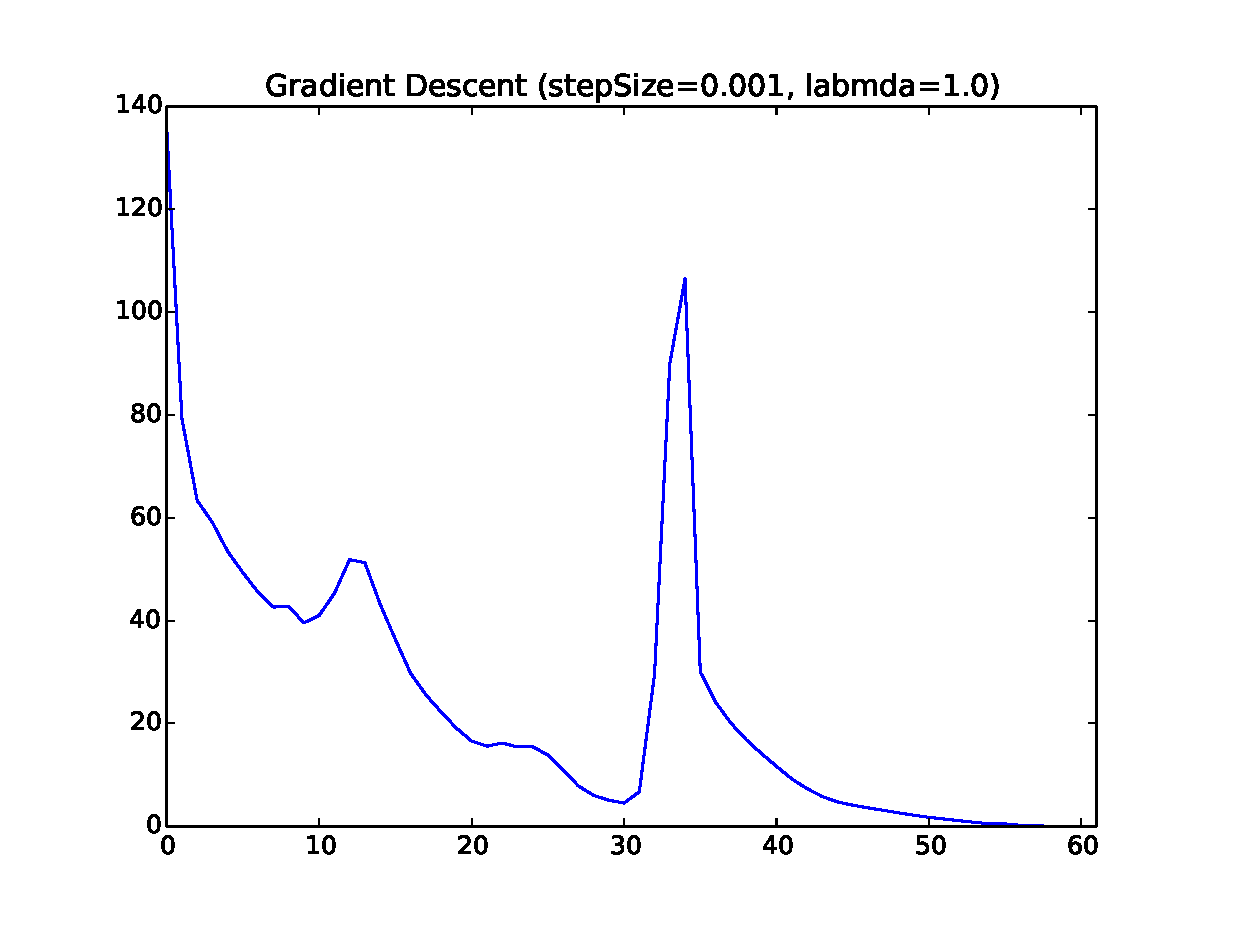
\includegraphics[width=120mm]{gradient_descent_large_lambda_1}
\caption{This figure shows the decrese in the objective over the iterations when $featureSet=2$, $stepSize=0.001$, and $lambda=1.0$.}
\label{fig:gradient_descent_large_lambda_1}
\end{figure}

For $stepSize$ and $lambda$, I employed a brute-force approach to find the best values. For each combination of $regularization$ and $featureSet$, I tried all the combination of $stepSize \in \{0.001, 0.01, 0.1\}$ and $labmda \in \{0.05, 0.1, 0.2, 0.4, 1.0, 2.0\}$ in order to find the optimal values that achieve the best accuracy on the validation data. One of the results are shown in Figure \ref{fig:performance_hyperparameter}. Notice that the performance significantly decreases when $lambda \ge 1$. This is resonable because the loss function becomes less important in the objective function. A large $lambda$ avoids overfitting but may deteriorate the performance, while a small $lambda$ can achieve better performance but may results in overfitting. Since we do not know the distribution of the test dataset beforehand, it is reasonable to use the performance on the validation data to choose values of $labmda$ as well as other hyperparameters. Note that if the distribution of the test dataset is significantly different from the validation dataset, then the selected values of hyperparameters cannot necessarily yield a good performance on the test dataset.

\begin{figure}[hbtp]
\centering
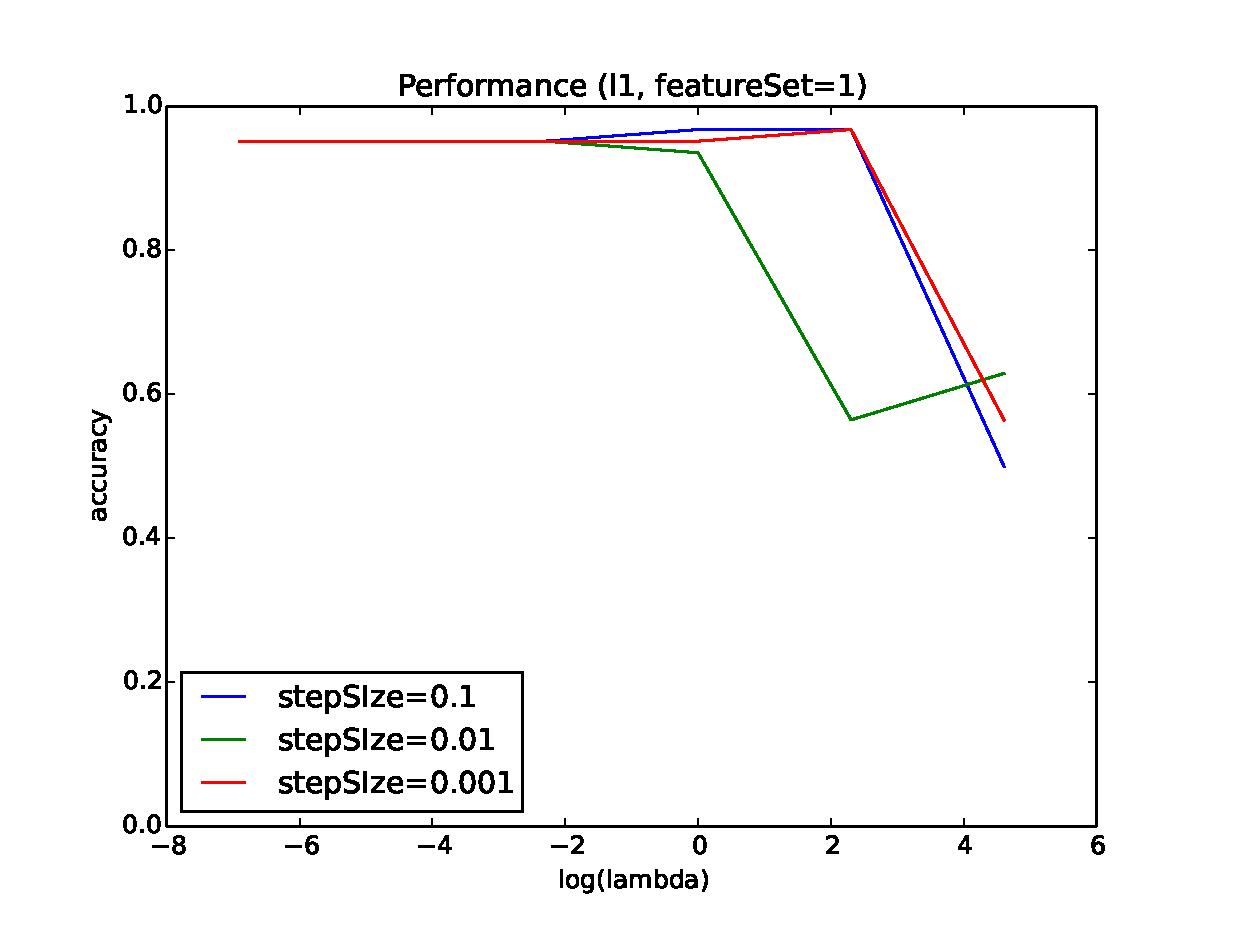
\includegraphics[width=150mm]{performance_hyperparameter}
\caption{This figure shows the accuracy over the validation data using different pairs of $stepSize$ and $lambda$ when $regularization=l2$ and $featureSet=1$. The performance drastically decreases when $lambda > 1$.}
\label{fig:performance_hyperparameter}
\end{figure}

The optimal values of $stepSize$ and $labmda$ that achieved the best performance on the validation data are listed in Table \ref{tab:best_hyperparameters}. For the following performance test, I used those values for hyperparameters.

\begin{table}[htb]
  \begin{center}
  \begin{tabular}{|c|c||c|c|} \hline
    featureSet & regularization & best stepSize & best  lambda \\ \hline
    1 & 11 & 0.001 & 0.4 \\ \hline
    1 & 12 & 0.001 & 0.4 \\ \hline
    2 & 11 & 0.001 & 0.1 \\ \hline
    2 & 12 & 0.001 & 0.2 \\ \hline
    3 & 11 & 0.001 & 0.05 \\ \hline
    3 & 12 & 0.001 & 0.1 \\ \hline
  \end{tabular}
  \caption{The best combination of $stepSize$ and $lambda$}
  \label{tab:best_hyperparameters}
  \end{center}
\end{table}

\subsection*{Results}
Using the selected values of $stepSize$ and $lambda$ for each $featureSet$ and $regularization$, the classifier was learned and the performance was evaluated on the training, validation, and test dataset. The results are shown in Tables 2-7. Note that the performance of $featureSet=2$ is very close to the one of $featureSet=3$. This implies that the feature pairs have much larger weighs than the original attributes when $featuerSet=3$ is used. Also, it is surprising that $featureSet=1$ yields the best performance. The possible reason is that the feature pairs cause the overfitting even though the regularizer is included in the objective.

\begin{table}[!h]
  \begin{center}
  \begin{tabular}{|c|c|c|c|c|c|c|c|c|} \hline
    dataset & accuracy & precision & recall & F1 \\ \hline
    training data & 1.0 & 1.0 & 1.0 & 1.0 \\ \hline
    validation data & 0.967 & 0.931 & 1.0 & 0.964 \\ \hline
    test data & 0.614 & 0.583 & 0.803 & 0.675 \\ \hline
  \end{tabular}
  \caption{The results of featurSet=1 with $l1$ regularization}
  \label{tab:result_1_l1}
  \end{center}
\end{table}

\begin{table}[!h]
  \begin{center}
  \begin{tabular}{|c|c|c|c|c|c|c|c|c|} \hline
    dataset & accuracy & precision & recall & F1 \\ \hline
    training data & 0.989 & 0.990 & 0.985 & 0.987 \\ \hline
    validation data & 0.967 & 0.931 & 1.0 & 0.964 \\ \hline
    test data & 0.598 & 0.571 & 0.786 & 0.662 \\ \hline
  \end{tabular}
  \caption{The results of featurSet=1 with $l2$ regularization}
  \label{tab:result_1_l2}
  \end{center}
\end{table}

\begin{table}[!h]
  \begin{center}
  \begin{tabular}{|c|c|c|c|c|c|c|c|c|} \hline
    dataset & accuracy & precision & recall & F1 \\ \hline
    training data & 1.0 & 1.0 & 1.0 & 1.0 \\ \hline
    validation data & 0.967 & 0.931 & 1.0 & 0.964 \\ \hline
    test data & 0.590 & 0.560 & 0.836 & 0.671 \\ \hline
  \end{tabular}
  \caption{The results of featurSet=2 with $l1$ regularization}
  \label{tab:result_2_l1}
  \end{center}
\end{table}

\begin{table}[!h]
  \begin{center}
  \begin{tabular}{|c|c|c|c|c|c|c|c|c|} \hline
    dataset & accuracy & precision & recall & F1 \\ \hline
    training data & 1.0 & 1.0 & 1.0 & 1.0 \\ \hline
    validation data & 0.967 & 0.931 & 0.1.0 & 0.964 \\ \hline
    test data & 0.606 & 0.573 & 0.836 & 0.680 \\ \hline
  \end{tabular}
  \caption{The results of featurSet=2 with $l2$ regularization}
  \label{tab:result_2_l2}
  \end{center}
\end{table}

\begin{table}[!h]
  \begin{center}
  \begin{tabular}{|c|c|c|c|c|c|c|c|c|} \hline
    dataset & accuracy & precision & recall & F1 \\ \hline
    training data & 1.0 & 1.0 & 1.0 & 1.0 \\ \hline
    validation data & 0.967 & 0.931 & 1.0 & 0.964 \\ \hline
    test data & 0.606 & 0.573 & 0.836 & 0.680 \\ \hline
  \end{tabular}
  \caption{The results of featurSet=3 with $l1$ regularization}
  \label{tab:result_3_l1}
  \end{center}
\end{table}

\begin{table}[!h]
  \begin{center}
  \begin{tabular}{|c|c|c|c|c|c|c|c|c|} \hline
    dataset & accuracy & precision & recall & F1 \\ \hline
    training data & 1.0 & 1.0 & 1.0 & 1.0 \\ \hline
    validation data & 0.967 & 0.931 & 1.0 & 0.964 \\ \hline
    test data & 0.606 & 0.573 & 0.836 & 0.680 \\ \hline
  \end{tabular}
  \caption{The results of featurSet=3 with $l2$ regularization}
  \label{tab:result_3_l2}
  \end{center}
\end{table}

\subsection*{Impact by the regularizer $l1$ and $l2$}
In general, $l1$ regularizer results in a sparse weight vector compared to $l2$ regularizer. To confirm this, for $featureSet=1$ I normalized the resulting weight vectors and compare them between $l1$ and $l2$. Out of 586 components of the weight vector, 313 components are zero when $l1$ regularizer is used, while only 287 componets are zero when $l2$ regularizer is used. This result confirms that $l1$ regularizer leads to a sparse weight vector. The sparsity is usually favorable because it leads to a simpler model, which indicates a more generalized model and requries less storage. Although it is known that $l1$ regularizer often leads to better performance in practice, there is usualy not a considerable difference between the two methods in terms of the accuracy of the resulting model \cite{gao2007, tsuruoka2009}. In fact, there is no significant difference in performace between $l1$ and $l2$ in the results.

\begin{thebibliography}{9}
\bibitem{gao2007} Gao, J., Andrew, G., Johnson, M., Toutanova, K. 2007. A comparative study of parameter estimation methods for statistical natural language processing. In {\it Proceedings of ACL}, pp. 824 - 831.
\bibitem{tsuruoka2009} Tsuruoka, Y., Tsujii, J., Ananiadou, S. 2009. Stochastic gradient descent training for l1-regularized log-linear models with cummulative penality. In {\it Proceedings of ACL}, pp. 477 - 485.
\end{thebibliography}

\end{document}

